\section{Introduction}

In this chapter, we provide a contextual overview of the modular robotic systems and their applications. In this dissertation, we primarily target large-scale ones \gls{lmrs}, namely the large-scale lattice-based modular robots composed of resource-constrained identical modules that communicate together using only neighbor-to-neighbor communications. This chapter offers a network characterization of those systems along with a discussion of the challenges involved in the design of distributed algorithms for such systems. Finally, we present our research environment, i.e., the hardware and simulation tools we use to apply and evaluate our research.

\section{Modular Robotics}

In this section we introduce modular robotics. We first define this concept. Then, we present the advantages offered by modular robotic systems.  Afterwards, we show some applications based on modular robotic systems. We then offer a classification of existing modular robotic systems. Finally, we discuss the network properties of \gls{lmrs}.

\subsection{Definition}

Over the past decades, modular robotics has emerged as a new way to design robotic systems. A modular robot is formed from independent, intelligent and communicating modules which act as a whole ensemble. It forms a distributed system in which modules cooperatively self-organize, perform specific tasks and achieve common goals. \acrfull{msr} can rearrange their global shape to adapt to a task or a given situation.

\subsection{Advantages over Traditional Robotics}

Compared to traditional robotic systems, \acrshort{msr}s have four main advantages: versatility, robustness, extensibility and low cost. The versatility property directly comes from the fact that an \acrshort{msr} can self-adapt to a specific, possibly unexpected, situation by rearranging its global morphology. This enables modules to perform a wide variety of different tasks, including tasks not even envisaged at the time of designing. Modules are interchangeable both inside a robot and potentially with some surrounding systems. Hence, modular robotic systems are more robust, they may self-repair in case of module failure by discarding or replacing faulty modules on the fly. Moreover, modular robotic systems can be scaled up by adding/deleting modules when necessary. In addition, they also have economic advantages as a wide variety of different and complex systems can be built from mass-produced modules.

\subsection{Examples of Potential Applications}

This section presents some interesting potential applications of modular robotic systems. To the best of our knowledge, none of the presented applications has been physically realized yet.

\paragraph{Conveyance System}
\label{section:context:conveyance-surface}

The Smart Blocks~\cite{piranda2013new} project aims to build a large distributed modular system to convey small and fragile objects, by attaching many modules together, each one equipped with a conveyance surface (see Figure~\ref{fig:context:conveyance-surface}). This surface can be deployed in inhospitable and remote locations (e.g., a remote planet, hazardous areas of a nuclear plant, etc.). The conveying system makes it possible to sort objects and transport them to different locations according to some criteria (e.g., shape, color, etc.). Moreover, if a module fails, the system can autonomously self-repair by replacing the faulty module by a functional one.

\begin{figure}[!h]
	\centering
	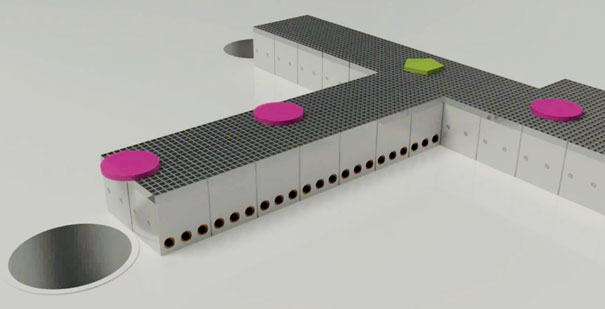
\includegraphics[width=0.5\linewidth]{images/context/conveyance-surface.jpg}
	\caption{Smart conveyance surface formed from Smart Blocks. The system sorts the objects it distributively conveyes. Purple circles and green hexagons are transported toward two different holes.}
	\label{fig:context:conveyance-surface}
\end{figure}

\paragraph{Programmable Matter}

\acrfull{pm} is a matter that can change its physical properties in response to external and programmed events. Different approaches and technologies to realize \gls{pm} are envisioned in the literature, e.g., \gls{pm} using 4D printing~\cite{tibbits20144d}, quantum wellstone~\cite{carthy2000programmable}, DNA structures~\cite{ke2012three,kim2011dna} and robotic-based approaches. The latter include the use of self-folding robots~\cite{Hawkes13072010}, tendon-driven robotic chains~\cite{lasagni2016dynamic}, robotic materials~\cite{mcevoy2015materials}, swarm robotic systems~\cite{rubenstein2014programmable} and modular self-reconfigurable robots~\cite{goldstein-waci04,GKR10}.

In the Clay-Electronics (Claytronics) project~\cite{goldstein-waci04}, it is envisioned to use large-scale micro modular robotic systems, composed of up to millions of modules called Claytronics Atoms (Catoms), to build \gls{pm}. Every Catom is a mass-producible micro robot that will have very restricted (i.e., strictly mandatory) functionalities. \gls{pm} promises synthetic reality and has a wide range of applications (e.g., sending/downloading copies of physical objects, morpheable objects reshapable at will, injectable surgical instruments, 3D interactive life-size TV, etc.). It will enable people not only to control their environment but also to shape it.

As shown in Figure~\ref{fig:context:pm-cup}, \gls{pm} offers, for instance, a drastic evolution of the computer-aided design process. In this vision, a computer holds a virtual representation of an object that can be transferred to some programmable matter in order to obtain a physical representation of that object. The virtual and the physical representations remain consistent at all times, i.e., if one changes, the other reflects this change. The user can modify the virtual representation and it will have an immediate impact on the physical representation of the object considered. He can also manually change the physical representation as he whishes, which will immediately update the virtual representation. Hence, designers will be able to simultaneously design a model and a prototype of their object, reducing significantly the time to prototype. Furthermore, the matter can be endlessly re-used and reshaped, thus this process will also minimize the waste of resources.

\begin{figure}[!h]
	\centering
	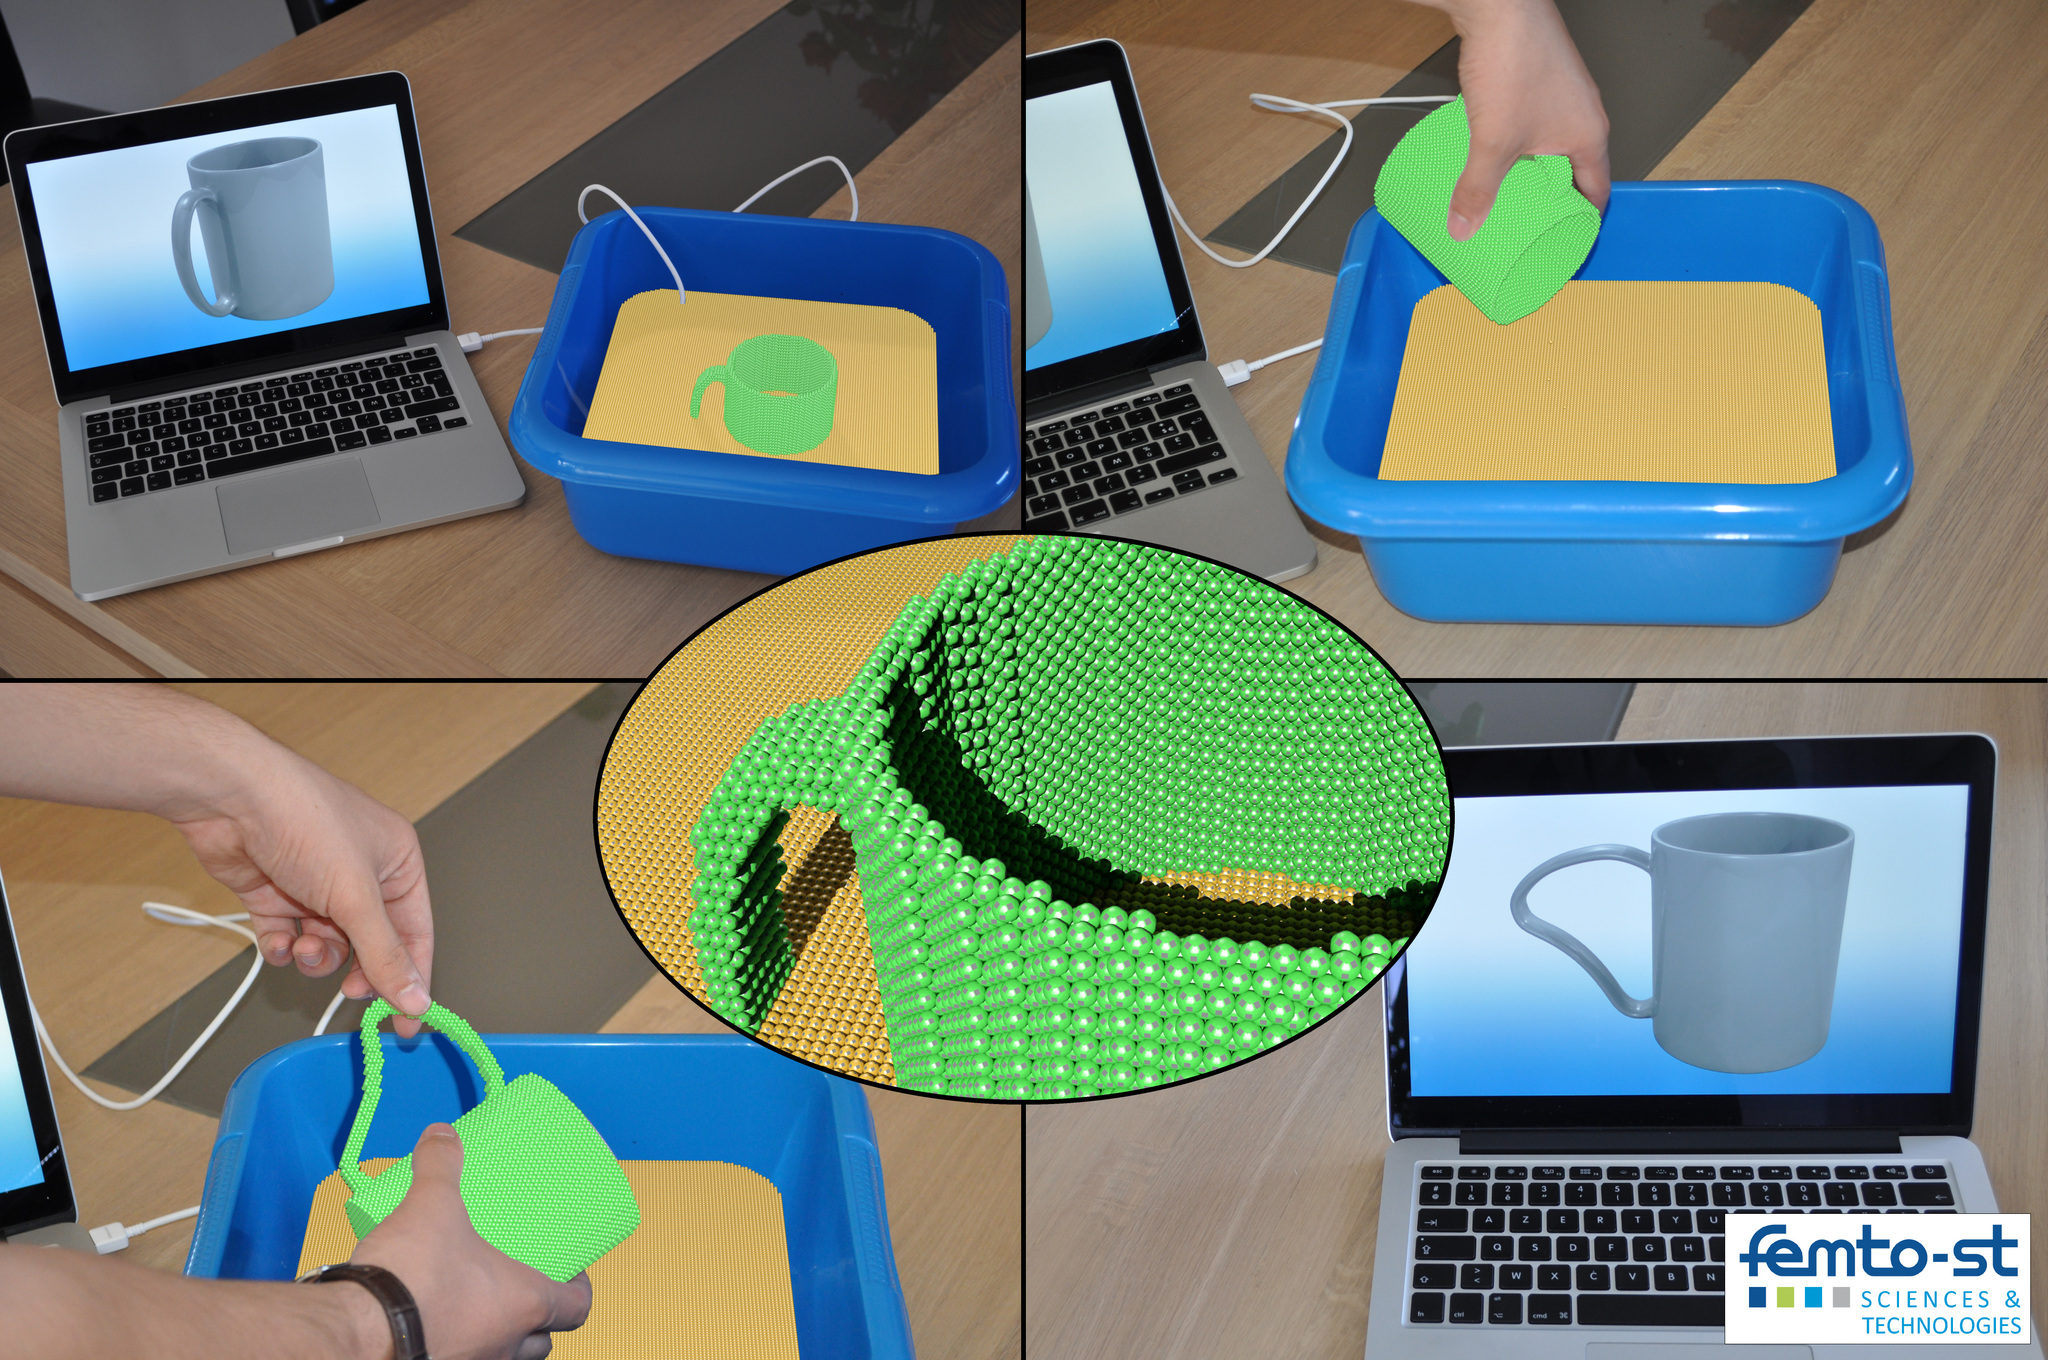
\includegraphics[width=0.7\linewidth]{images/context/cup.jpg}
	\caption{Programmable matter as a cyber-physical conjugation to enhance the computer-aided design process (from~\cite{bourgeois-smc2016}). The cyberized representation of a cup is transferred to the matter composed of hundreds of thousands of modules. The physical representation is then manipulated and manually modified. The cyberized representation remains consistent with the physical one and reflects the change.}
	\label{fig:context:pm-cup}
\end{figure}

\paragraph{Space Exploration}

Modular robotic systems can be used to overcome volume limitations in spacecraft during space exploration missions as explained in~\cite{yim2009modular}. Modules can be packed in a dense way in order to meet vessel volume constraints and deploy at will during a mission to perform different tasks. Moreover, MSR-based objects can potentially self-repair, thus limiting the risk of a mission aborting in case of critical-equipment failure.

\paragraph{Search and Rescue}

Modular robotic systems may also be used in search and rescue operations in collapsed buildings, as explained in~\cite{yim2009modular}. For instance, an MSR system can transform its shape to sneak in ruins and pass through narrow passages in order to locate victims. Once a victim is found, the robot can emit a signal with its position and take the form of a shelter to protect the victim until rescued.

\subsection{Existing Systems and Classification}
\label{section:context:classification}

Existing modular robotic systems differ by their architecture (e.g., lattice, chain, mobile), their communication model (e.g., neighbor-to-neighbor communication, global communication through a shared medium, hybrid model), their module and overall scale (nanometer, micrometer, millimeter, centimeter, meter, etc.), their sensing and actuation (self-reconfigurable, manually reconfigurable, etc.) capabilities, etc. A comprehensive overview of the existing modular robotic systems can be found in surveys~\cite{chennareddy2017modular, Ahmadzadeh:2016:MRS:2893814.2893968,yim2007modular}. The complexity that lies in the coordination of large-scale modular robotic systems depends on these hardware parameters~\cite{yim2009modular}.

In lattice-based modular robots, modules are arranged in some regular 2-dimensional or 3-dimensional lattice structures. In chain-based structures, modules are connected together in a serial manner forming an articulated chain or tree. By contrast, in mobile architectures, modules are free to move in the continuous space and can dock together to form lattice, chain or free structures.

In the neighbor-to-neighbor communication model, modules communicate only with adjacent modules. This communication model is fundamentally different than the global communication model where all modules can directly communicate together, for example, through a global bus. The later approach works well in small networks, but it is not scalable. Indeed, packet collisions may frequently occur. Moreover, if the shared communication medium is a bus, the number of hosts it can support is limited. Some hybrid approaches have been proposed but they are not common in modular robotics and complex to implement in a resource-constrained environment.

%\glsreset{lmrs}
In this dissertation, we focus our attention on lattice-based modular robots composed of identical resource-constrained modules that communicate together using only neighbor-to-neighbor communications. We name this class of modular robotic systems \gls{lmrs}. As shown in~\cite{bourgeois-smc2016}, \acrshort{lmrs} are particularly suitable to realize large-scale ensembles of modular robotic systems (e.g., Claytronics \gls{pm}). Moreover, the class of modular robots considered captures a variety of existing systems, e.g., the Telecubes~\cite{suh2002telecubes}, the Miche~\cite{gilpin2008miche} and the Distributed Flight Array~\cite{oung2011distributed} modular robots, some of the self-assembling systems used in~\cite{bhalla2007framework} and most of the modular robotic systems developed in the Smart Blocks and the Claytronics projects. Figure~\ref{fig:context:modular-robots} shows some \gls{lmrs} developed in these two projects, namely the Smart Blocks, the millimeter-scale 2D Catoms, the Blinky Blocks and the 3D Catoms~\cite{piranda2016geom}. These modular robots are respectively arranged in the square, the hexagonal, the simple cubic, and the face-centered cubic lattices.

\begin{figure}[!h]
	\centering
	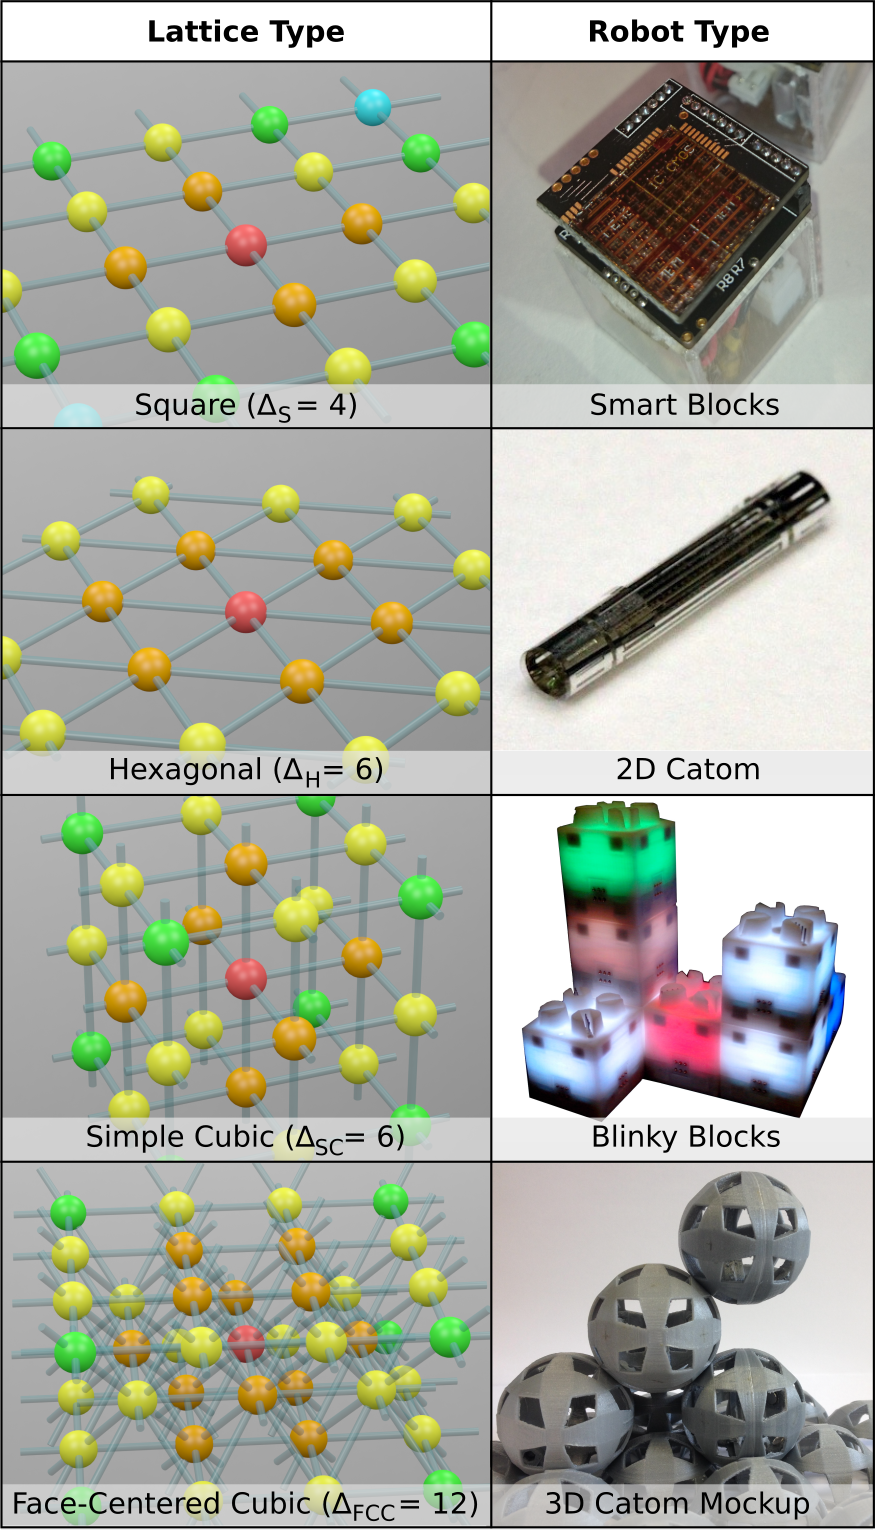
\includegraphics[width=0.55\linewidth]{images/network-characterization/types.png}
	\caption{Different lattice arrangements associated with modular robotic systems developed in the Smart Blocks and the Claytronics projects. For a lattice $L$, $\Delta_L$ denotes its coordination number, i.e, the maximum number of modules to which a module can be connected.}
	\label{fig:context:modular-robots}
\end{figure}

\subsection{Network Properties of Large-Scale LMRs}
\label{section:context:lmrs}

In this section, we present key network characteristics of large-scale \gls{lmrs} and discuss the challenges implied by these properties in the design of efficient distributed algorithms for large-scale ensembles.

\begin{description}
	
	\item[Restricted Resources] Nodes are low-cost small electronic devices. Thus, they are equipped with limited capabilities. They have scarce computation, memory and energy resources. They may also have, for instance, low-precision clocks making distributed real-time control a difficult task. 
	
	\item[Asynchrony] Modules of \gls{lmrs} are inherently asynchronous. Indeed, there is no global clock and every module processes independently of the others. In particular, communication between modules is asynchronous.
	
	\item[Neighbor-to-Neighbor Communications] In the neighbor-to-neighbor communication model, a module uses a separate network interface and communication channel for each of its neighbors. The network has neither local nor global shared broadcast medium. A remarkable advantage of the absence of shared communication medium is that we do not have to deal with potential network collisions. In our model, a module can communicate simultaneously with all its neighbors. Moreover, in order to locally broadcast a message, a module has to send an individual copy of that message to all neighbors. Although trivial, these two properties have to be taken into account when designing algorithms at risk of overwhelming the network. For instance, if all nodes simultaneously start a network flooding operation, a node may generate messages at a higher rate than it can send them. A node may receive a message per neighboring node in a short amount of time, thus adding several messages in the channel to each of its other neighbors. A short amount of time later, the same node might again receive a message from all its neighbors and add messages in its outgoing message queues, although only a part of the messages previously inserted into the outgoing queue has been sent. Thus, messages progressively pile up. If this situation occurs several times, the outgoing queues keep growing and the network gets congested. This issue is further discussed in Section~\ref{section:centrality-controlled-broadcast}.	

	\item[Sparse Networks]  We demonstrate in Appendix~\ref{appendix:lmrs} that \gls{lmrs} form sparse networks, i.e., $m \ll n^2$, where $n$ is the number of modules in the system and $m$ the number of links in the network. Moreover, we show that the number of links is $\Theta(n)$. We compare lattice-based networks to small-world networks~\cite{watts1998collective} (e.g., the Internet network~\cite{jin2006small}) and to wireless ad-hoc networks (e.g., wireless sensor networks, multi-robot networks, etc.). Since many large real-world networks are small-world networks, it is legitimate to consider them for comparison. Wireless ad-hoc networks are highly spatially dependent, like our class of networks. Indeed, in wireless ad-hoc networks, nodes can only communicate with some neighboring nodes within some limited range. Note that wireless ad-hoc networks can fall in the class of lattice-based networks if they are deployed in a lattice structure. Lattice-based networks are sparser than small-world networks that have $\Omega(n\log(n))$ edges~\cite{watts1998collective}. Wireless ad-hoc networks can be sparse or dense, depending on the deployment environment (area/volume, obstacles, etc.), the deployment density and the node communication range. An example of sparse sensor network is the 46-hop network of 64 sensors deployed in a long-linear topology on the Golden Gate Bridge, in San Francisco (United States), in order to monitor the effects of wind and earthquakes on the structure~\cite{kim2007health}.

	\item[Large Hop Distances] In systems where nodes use neighbor-to-neighbor communications, the node spatial arrangement directly reflects the connectivity graph. Modular robotic systems often have a bounded number of connectors, i.e., of potential neighbors. As a direct consequence, large-scale modular robotic ensembles tend to exhibit large hop distances. Due to the regular tiling of the space in lattices, networks of \gls{lmrs} obey certain geometric rules. In regular lattice networks, the typical distance between two nodes is $\sim {n}^{\frac{1}{D_L}}$~\cite{barthelemy2011spatial} where $D_L$ is the geometric dimension of the lattice $L$. Thus, in lattice-based networks, i.e., lattice networks with potential holes, this distance is lower bounded by $\Omega({n}^{\frac{1}{D_L}})$, while in small-world networks, this distance is $\sim log(n)$~\cite{barthelemy2011spatial}. In Appendix~\ref{appendix:lmrs}, we provide exact bounds on the radius and the diameter of these networks based on their lattice type and the number of modules in the system.  Moreover, we demonstrate that the radius and the diameter of lattice-based networks are lower bounded by $\Omega(\sqrt[3]{n})$. Small-world networks have typically short distances between arbitrary pairs of nodes due to the presence of a few long-range edges. As a consequence, small-world networks tend to have a small diameter. In lattice-based and sparse wireless ad-hoc networks, such long-range edges do not exist. Thus, these networks tend to have a larger average distance and a larger diameter. These phenomena are accentuated as the number of nodes in the network increases. 
	Studies indicate that the diameter of the Internet is around 30 hops~\cite{latapy2006measuring,leguay2005describing,cardozoend}. This is corroborated by the suggested values for Time-To-Live (TTL) for Internet Protocol (IP) packets. The TTL should be twice the diameter of the Internet~\cite{rfc1122} and the actual value recommended is 64~\cite{rfc1700,iana}. As shown in Figure~\ref{fig:context:bounds}, systems with a million 3D Catoms have a diameter of at least 132 hops, while systems with 100 million 3D Catoms have a diameter of at least 620 hops. Similarly, Blinky Blocks systems have a large diameter, e.g., a 40,000 Blinky Blocks system has a diameter greater than 30 hops. Thus, a 40,000 Blinky Blocks system which fits in a $1.4\ m^3$ cube, would have a diameter larger than the entire Internet that spans the whole world. It is crucial to take into account the large diameter and large average distance to design efficient and effective distributed algorithms for large-scale modular robotic systems. For example, communication over a large number of hops causes latency and reliability issues. Let us consider time synchronization and data sharing algorithms. These algorithms are, for instance, required for real-time responsive programmable matter and to distribute, store and access geometry data for self-reconfiguration. However, these algorithms are challenging to design for such large-diameter and large-average-distance systems. Unpredictable delays (due, for example, to queueing or retransmissions) accumulate every hop, which tends to disturb the time synchronization process and decrease the achievable synchronization precision. Moreover, in data sharing algorithms, lookup latency may be extremely long if it involves messages that have to travel a large number of hops.
\end{description}

\begin{figure}[!h]
	\centering
	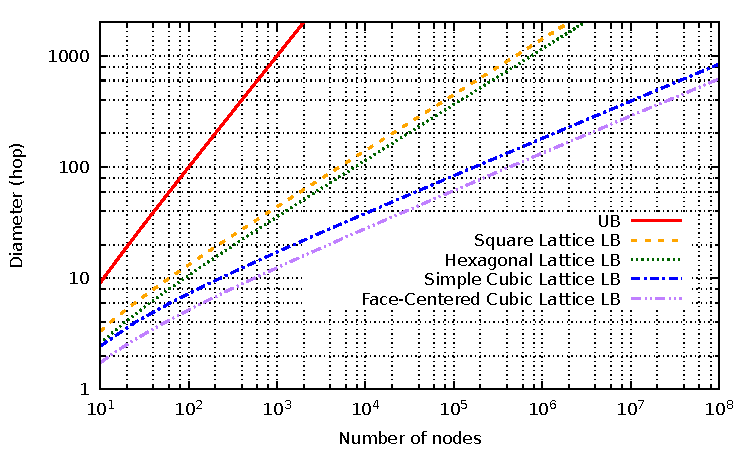
\includegraphics[width=0.9\linewidth]{images/network-characterization/bounds}
	\caption{Diameter bounds versus the number of nodes in the network for the different lattices considered. The terms \inquote{LB} and \inquote{UB} respectively stand for \inquote{lower bound} and \inquote{upper bound}.\label{fig:context:bounds}}
\end{figure}

\section[Research Environment: Evaluation Hardware and Simulation Tools]{Research Environment: Evaluation Hardware and Simulation Tools%
	\sectionmark{Research Environment: Evaluation Hardware and Simula...}}
\sectionmark{Research Environment: Evaluation Hardware and Simula...}
\label{section:context:environment}

This section presents the hardware and simulation tools we use to apply and evaluate the contributions introduced in this thesis. We consider the Blinky Blocks~\cite{Kirby-chi11} and the 2D Catoms~\cite{karagozler-iros09,karagozler-phdthesis} modular robotic systems. We first present technical features of these two systems.

In the next chapters, we evaluate our algorithms using both hardware prototypes and simulations. We have at our disposal several dozens of hardware Blinky Blocks to perform experimental evaluations. In order to carry out evaluations on 2D Catoms systems and on large-scale Blinky Blocks systems, we use VisibleSim~\cite{dhoutaut2013efficient}, our simulator of modular robotic systems. This section also presents VisibleSim.

\subsection{Blinky Blocks}
\label{section:context:blinkyblocks}

Blinky Blocks are centimeter-size blocks that were developed in the Claytronics project. Figure~\ref{fig:context:blinkyblocks} shows the details of a single block and an example of program running on an ensemble of hardware Blinky Blocks. We have at our disposal a few dozen Blinky Blocks to evaluate our algorithms on real hardware.

\begin{figure}[!h]
	\centering
	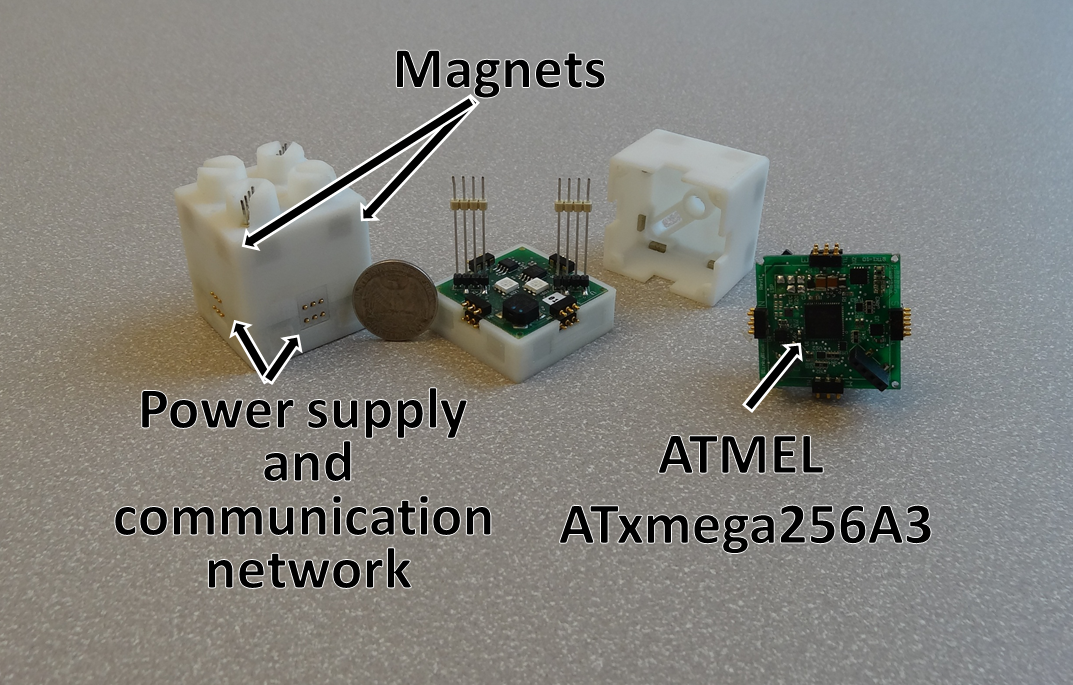
\includegraphics[width=0.475\linewidth]{images/context/bb-details.png}
	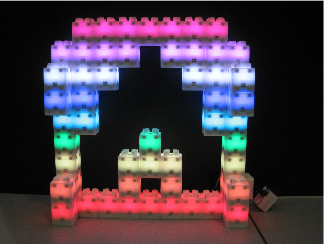
\includegraphics[width=0.475\linewidth]{images/context/bb-rainbow.png}
	\caption{On the left, dissection of a Blinky Blocks hardware prototype. On the right, an ensemble of 58 Blinky Blocks hardware prototypes running the Rainbow program (from~\cite{Kirby-chi11}). In the Rainbow program, blocks are colored depending on their level in the structure.}
	\label{fig:context:blinkyblocks}
\end{figure}

Blocks are attached to each other using magnets. Each module has its own computational power provided by an ATMEL ATxmega256A3-AU 8/16-bits 32-MHz micro-controller having 256KB ROM and 16KB RAM~\cite{xmegaA3datasheet}, as well as sensors and actuators such as RGB leds to glow with different colors according to the programmer's will.

All the blocks of a system execute the same program. A single block is connected to a power supply. Power is distributed through the system using dedicated pins. A block can have up to 6 neighbors and can communicate with them through serial links on the block faces. Ensembles of Blinky Blocks are manually reconfigurable at will. Blinky Blocks use full-duplex neighbor-to-neighbor communications over serial links controlled by Universal Asynchronous Receivers/Transmitters (UARTs) configured with a bitrate of 38.4~kBauds. Modules exchange frames that contain up to 17~bytes of data. Furthermore, a distributed logging system enables all modules to send information to a computer connected to the system using a serial connection.

More details on the Blinky Blocks communication system along with the characteristics of the block hardware clocks are provided in Section~\ref{section:time-sync:target}.

\subsection{2D Catoms}
\label{section:context:catom2D}

2D Catoms are millimeter-scale cylindrical robots~\cite{karagozler-iros09,karagozler-phdthesis} developed in the Claytronics project. 2D Catoms have been partially validated with the realization of a hardware prototype (see Figure~\ref{fig:context:catom2D}).

\begin{figure}[!h]
	\centering
	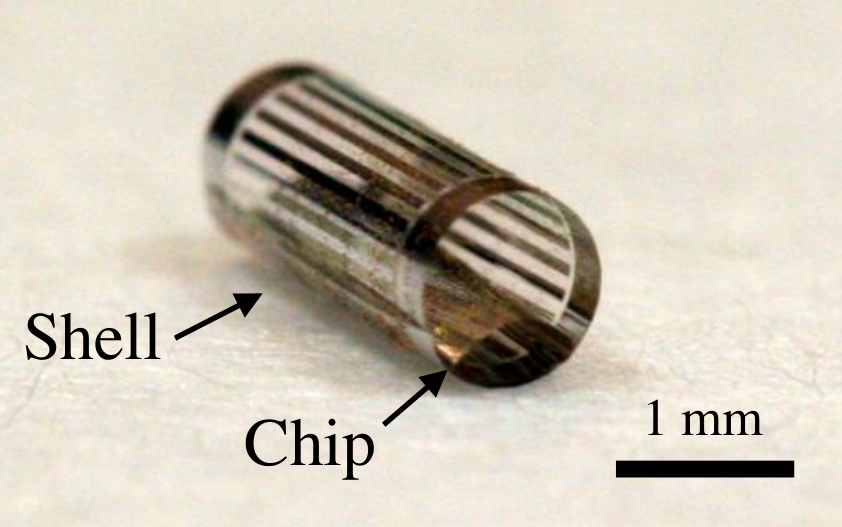
\includegraphics[width=0.35\linewidth]{images/context/catom_fabricated.png}
	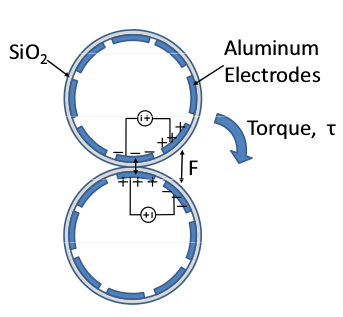
\includegraphics[width=0.35\linewidth]{images/context/catom_actuation.png}
	\caption{2D-Catom prototype (from~\cite{karagozler-phdthesis}).}
	\label{fig:context:catom2D}
\end{figure}

A 2D Catom consists of a 6-mm long-and 1-mm-diameter cylindrical shell. A high-voltage CMOS die is attached inside the tube. The chip includes a storage capacitor and a simple logic unit. The tube has electrodes used for power transfer, communications and actuation. 

In our work, we assume the power is spread from a powered floor through the ensemble using neighbor-to-neighbor power transfer. We consider that 2D Catoms are organized into a horizontal pointy-topped hexagonal lattice where modules have up to six neighbors. Modules can communicate together using neighbor-to-neighbor communications. 

Moreover, a 2D Catom can roll \acrfull{cw} or \acrfull{ccw} around a stationary module. During an atomic move, a module rotates $60°$, going from one cell of the lattice to its adjacent cell. We assume that a 2D Catom has only the capability to lift itself, it cannot carry or push other modules. In the current design, a 2D Catom is theoretically able to perform a revolution in 1.67 seconds or 3.35 seconds~\cite{karagozler-phdthesis}, which corresponds to an average speed\footnote{Let $t_r$ and $t_u$ respectively denote the time for a complete revolution and the time for a unit movement. In a revolution, a $d$-millimeter diameter cylindrical catom horizontally travels $\pi d$ millimeters. Hence, $v = \frac{d\pi}{t_r}$. For $t_r = 1.67s$, $v = \frac{d\pi}{t_r} = 1.88 mm \cdot s^{-1}$. In a unit movement, this catom travels $\frac{1}{6} \times \pi d = 0.523 mm$. Thus, $t_u = \frac{0.523}{v}$. Note that $t_u$ can be computed without determining $v$. Indeed, $t_u = t_r \times \frac{60}{360}$. For $t_r = 1.67 s$, $t_u = 0.278s$.} of $1.88~mm \cdot s^{-1}$ or $0.94~mm \cdot s^{-1}$.

%http://www.education.rec.ri.cmu.edu/previews/rcx_products/robotics_educator_workbook/content/mech/pages/Diameter_Distance_Traveled.pdf

\subsection{VisibleSim}
\label{section:context:visiblesim}

The VisibleSim simulator~\cite{dhoutaut2013efficient} is a discrete-event simulator for modular robots developed in our team (see Figures~\ref{fig:context:visiblesim-blinkyblocks-abccenter} and ~\ref{fig:context:visiblesim-catoms2D-c2sr}).

\begin{figure}[!h]
	\centering
	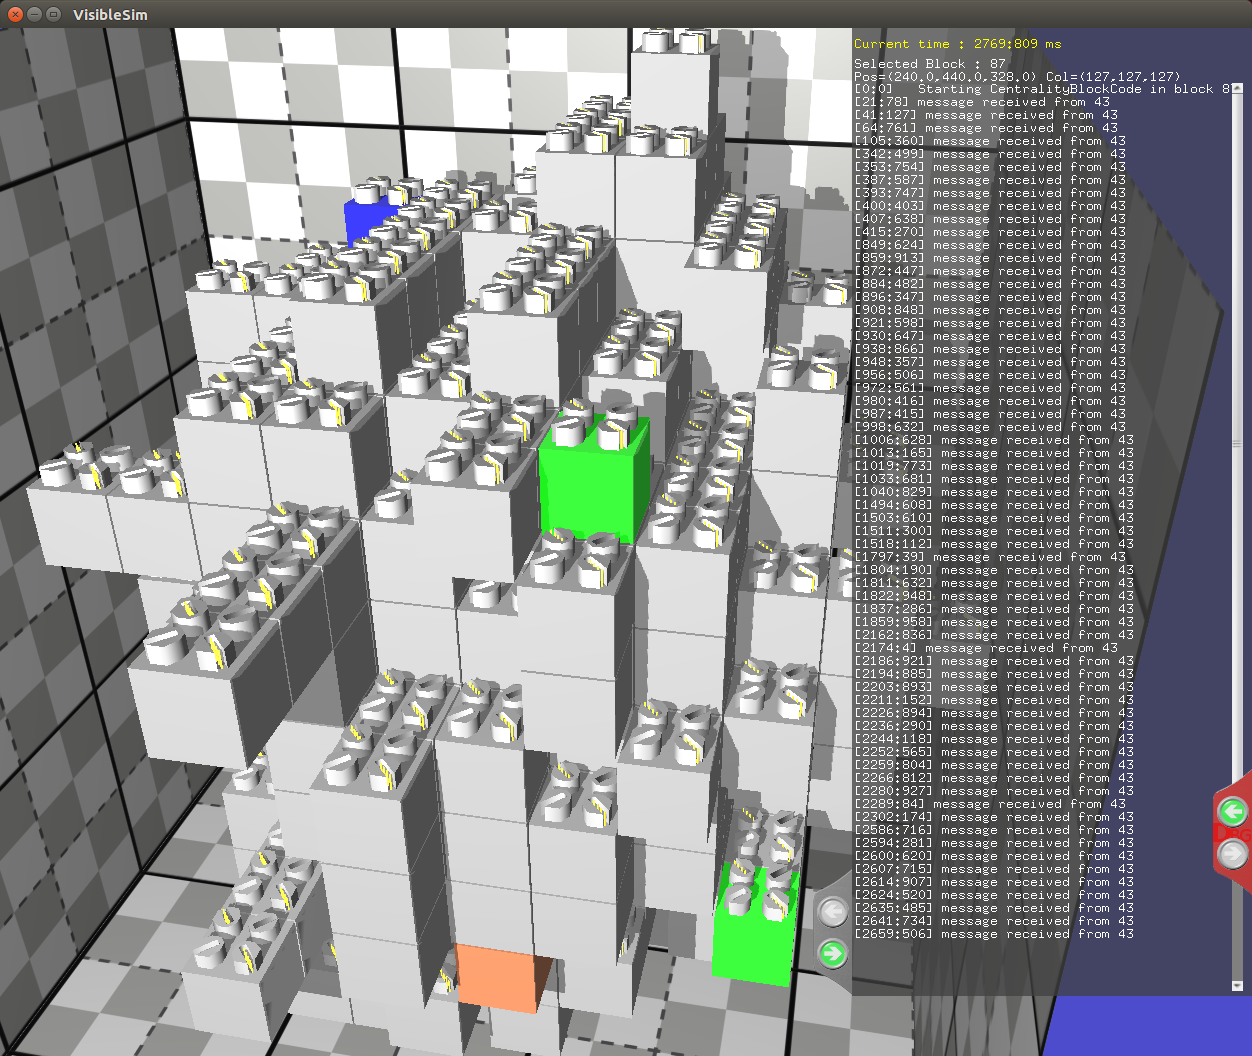
\includegraphics[width=0.85\linewidth]{images/context/visiblesim-abc-center.png}
	\caption{Screenshot of VisibleSim simulating the execution of the ABC-CenterV1 algorithm (see Section~\ref{section:centrality:abc-center}) in an ensemble of 500 Blinky Blocks.}
	\label{fig:context:visiblesim-blinkyblocks-abccenter}
\end{figure}

\begin{figure}[!h]
	\centering
	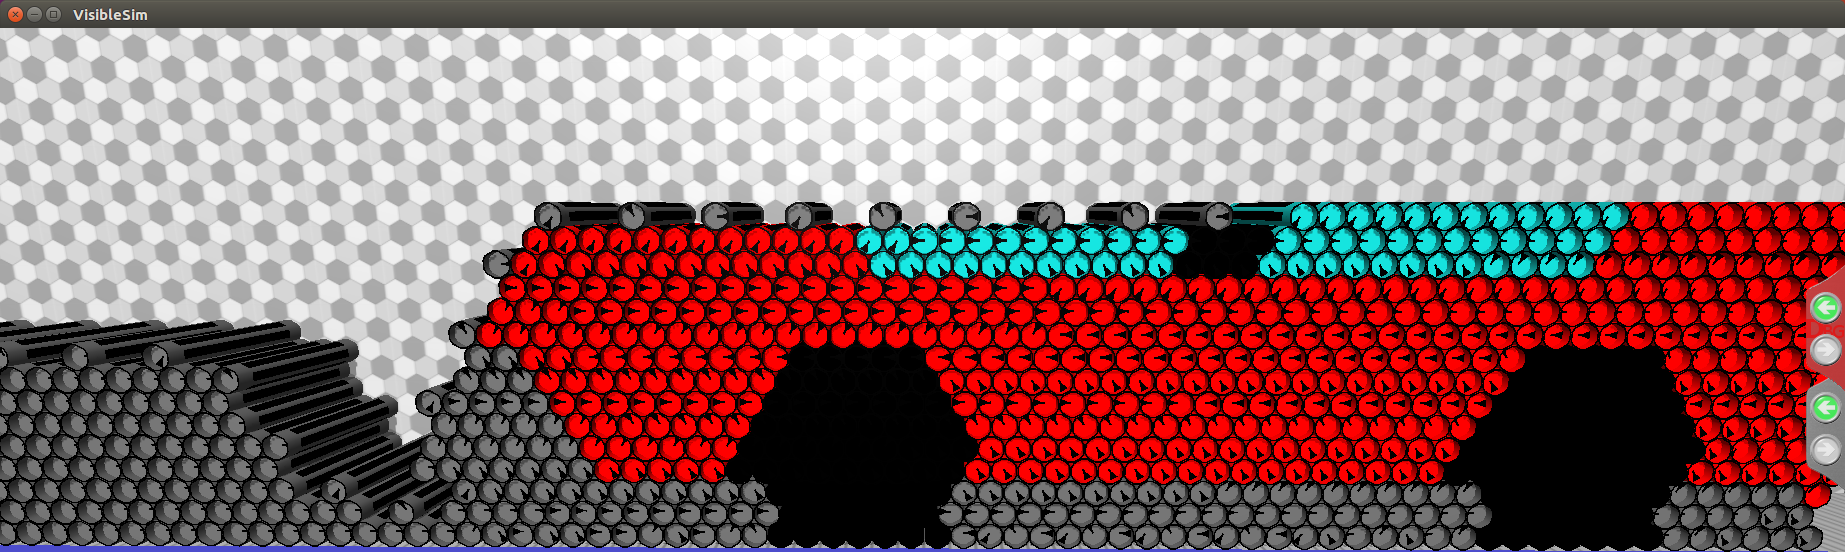
\includegraphics[width=\linewidth]{images/context/visiblesim-c2sr.png}
	\caption{Screenshot of VisibleSim simulating the execution of the Cylindrical Catoms Self-Reconfiguration (C2SR) algorithm in an ensemble of 1073 2D-Catoms (see Section~\ref{section:reconfiguration:at-a-glance}).}
	\label{fig:context:visiblesim-catoms2D-c2sr}
\end{figure}

VisibleSim supports a variety of different modular robotic systems (e.g., the Blinky Blocks, the 2D Catoms, the Smart Blocks, the 3D Catoms). We use VisibleSim to simulate the behavior of algorithms on modular robotic ensembles and also to benchmark their performance in terms of execution time, communications, number of motions, etc. 

VisibleSim enables to perform experiments on large-scale ensembles as it can handle simulations with dozens of thousands of modules. VisibleSim also allows us to carry out experiments on modular robotic systems for which we do not have fully functional hardware prototypes at our disposal (e.g., the 2D Catoms).

To properly simulate system asynchrony, VisibleSim can be run with variable motion and communication models. The simulation models used in the evaluation of the contributions of this thesis are chapter-specific and thus detailed later on in the evaluation section of the different contribution chapters.

\section{Conclusion}

In this chapter, we provide a short overview of modular robotics. In addition, we present the hardware and simulation tools we use to apply and evaluate the contributions introduced in this thesis.

Moreover, we show that large-scale \gls{lmrs} form asynchronous, low-degree, sparse, large-average-distance and large-diameter networks. In addition, units have limited computation, memory and energy resources. It is important to take into account these properties to design efficient and effective distributed algorithms for large-scale ensembles. In the next chapter, we propose algorithms to distributively elect a central module that is well located to communicate with all the others.